\documentclass[11pt]{article}
\usepackage{fullpage}
\usepackage{setspace}
\usepackage{amsmath}
\usepackage{fancyvrb}
\usepackage{enumerate}
\usepackage{pgfplots}
\usepackage{graphicx}
\usepackage{float}
\usepackage{multirow}
\usepackage[format=hang,labelsep=quad]{caption}
\usepackage{subfig}
\usepackage{array}
\usepackage{multirow}

\renewcommand\thesubfigure{\roman{subfigure}}


\begin{document}
\noindent\large{Math 5365}\\
\large{Data Mining 1}\\
\large{Homework 18}\\
\large{Mary Barker}
\doublespace
\begin{enumerate}
\item 
 Consider the data from problem 1 on Homework 17 

\begin{enumerate}
\item
 Find the number of clusters that maximizes the silhouette coefficient, 
 and plot the silhouette coefficient, and plot the silhouette 
 coefficient vs K. 

\begin{center}
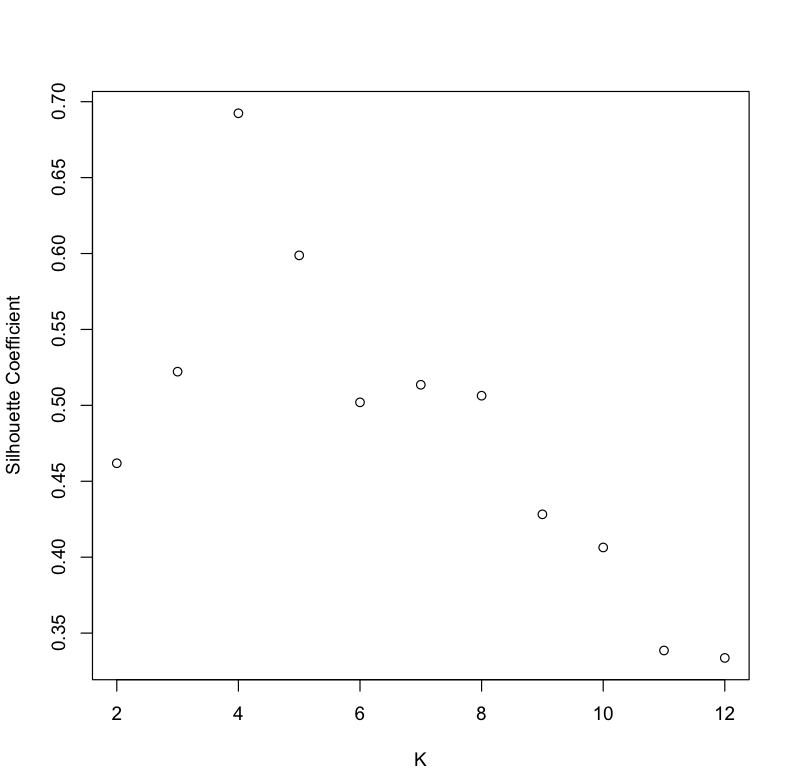
\includegraphics[scale=0.35]{pix/silhouette_k}
\end{center}

The optimal number of clusters for the silhouette coefficient is 4.


\item What is the maximum possible value of the silhouette coefficient? 
\begin{Verbatim}
$max
[1] 0.6923732

$where
[1] 4
\end{Verbatim}


\item
 Plot SSW vs K. Does the optimal value of K suggested by this plot agree 
 with the one based on the silhouette coefficient? 

\begin{center}
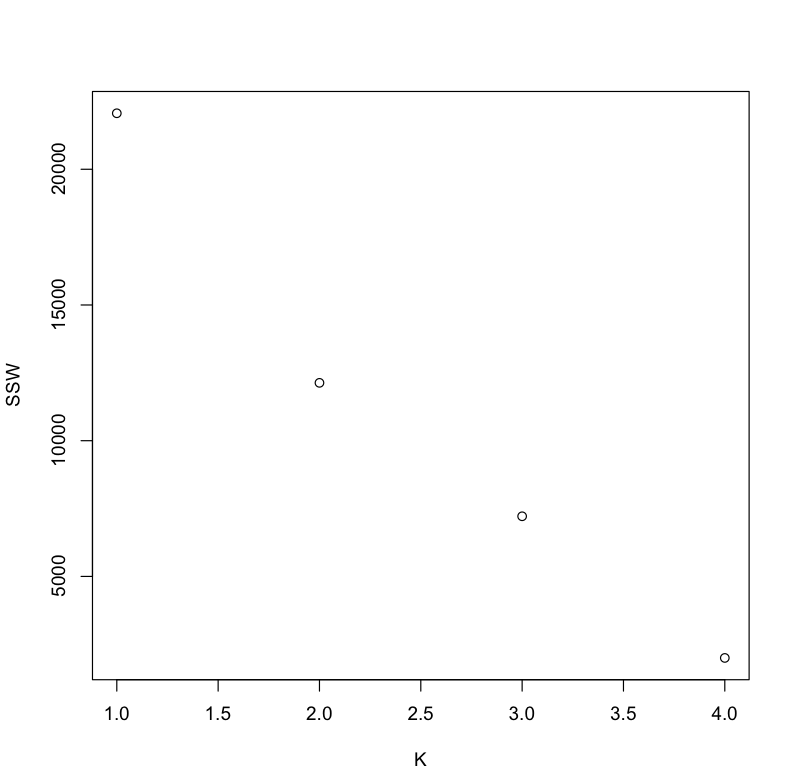
\includegraphics[scale=0.35]{pix/ssw_k}
\end{center}

\item
 Optional: Is the silhouette cofficient for this clustering statistically 
 significant? (It may be a good idea to let R run while you're out of the 
 office to do this problem.)

Running the same case with uniform data gave a silhouette coefficient maximized at 
k = 4 also. 

\begin{Verbatim}
$max
[1] 0.4182791

$where
[1] 4
\end{Verbatim}

\begin{center}
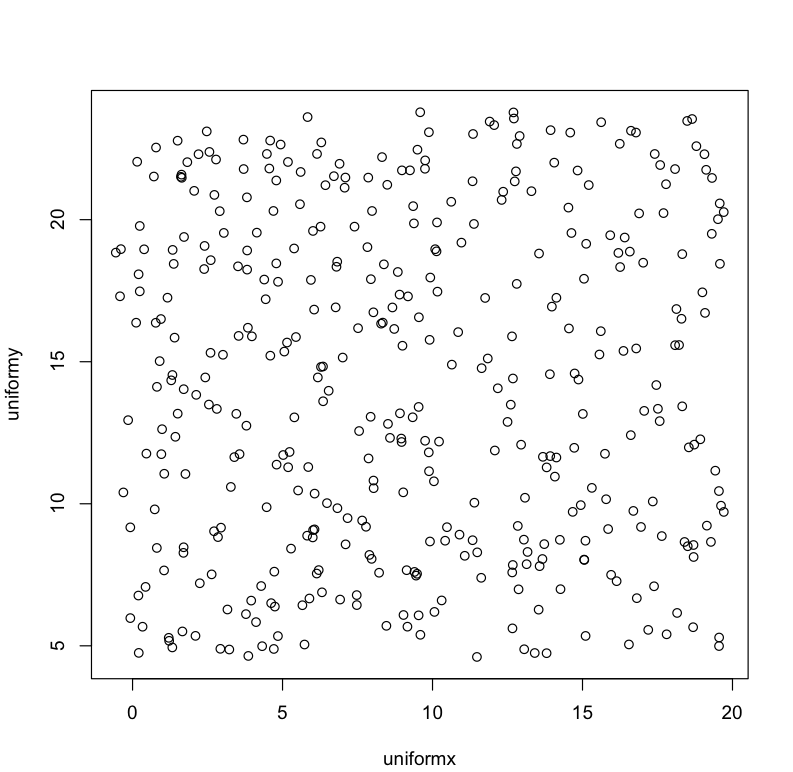
\includegraphics[scale=0.35]{pix/uniform_pts}
\end{center}

\begin{center}
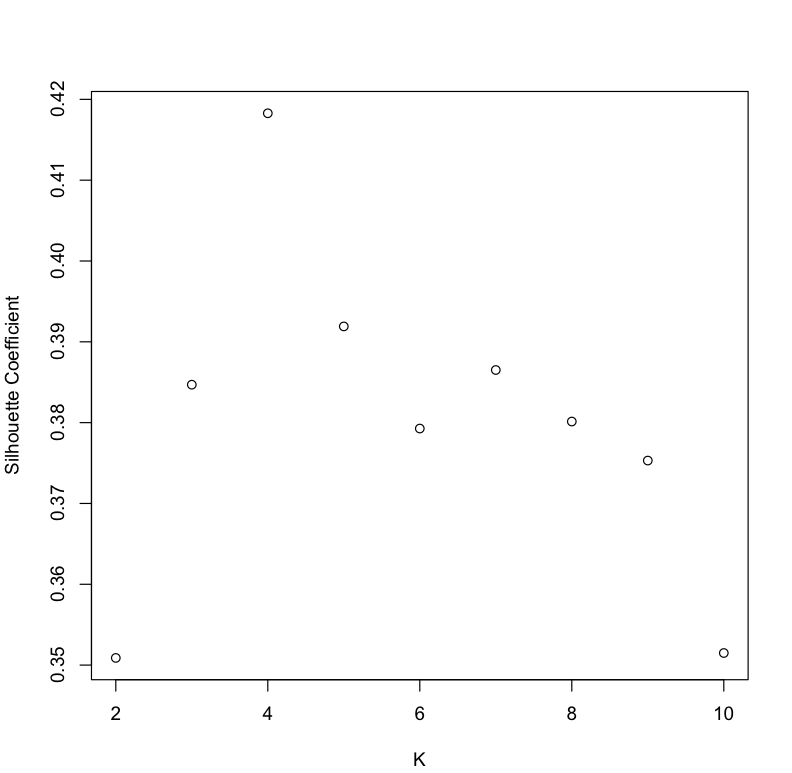
\includegraphics[scale=0.35]{pix/silhouette_for_uniform}
\end{center}

\end{enumerate}

\item 
 Repeat problem 1 for the wdbc data set. Also, find the weighted entropy 
 and purity for the optimal clustering. 

\begin{Verbatim}
$max
[1] 0.6972646

$where
[1] 2
\end{Verbatim}

\begin{center}
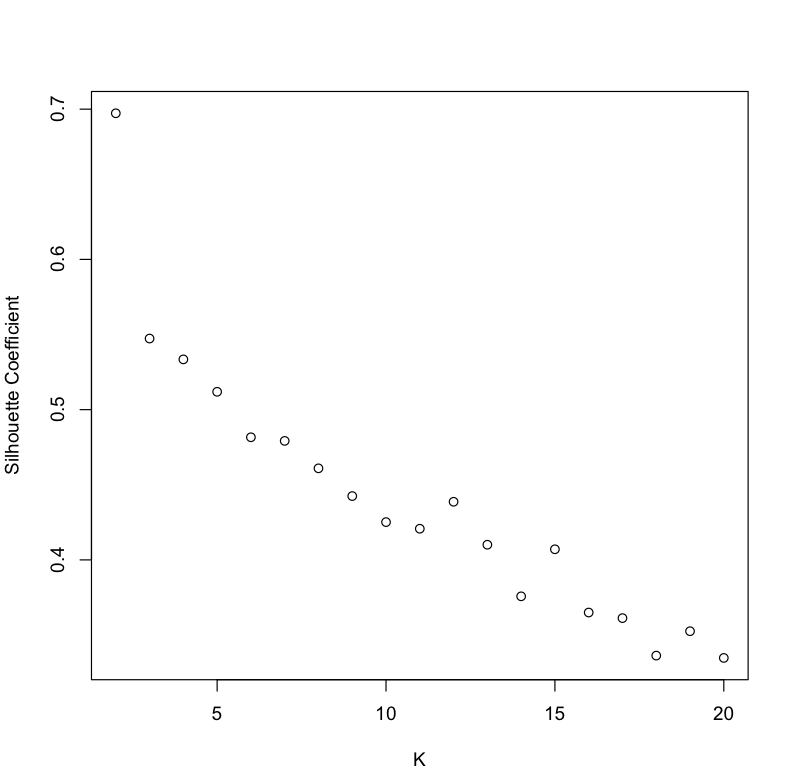
\includegraphics[scale=0.35]{pix/sil_vs_k}
\end{center}

\begin{center}
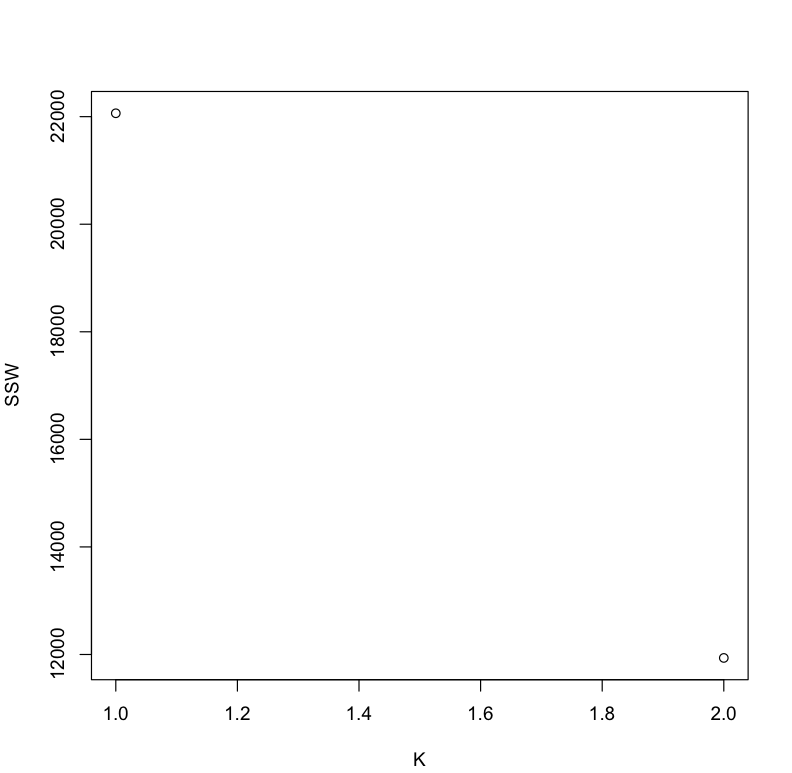
\includegraphics[scale=0.35]{pix/ssw_}
\end{center}

entropy = 0.5503462

purity = 0.8541301

\end{enumerate}
\singlespace
\begin{Verbatim}[numbers=left]
#Data Mining hw 18
library(stats)
library(cluster)
library(fields)

wdbc <- read.csv('~/Dropbox/Tarleton/data_mining/dfiles/wdbc.data',
                 header=F,sep=',')
wdbc <- wdbc[,-1]
source('~/Dropbox/Tarleton/data_mining/generic_functions/dataset_ops.R')
source('~/Dropbox/Tarleton/data_mining/generic_functions/measures.R')

x <- c(rnorm(100,  5, 1.5), rnorm(100, 15, 1.5), 
       rnorm(100,  5, 1.5), rnorm(100, 15, 1.5))
y <- c(rnorm(100, 10, 1.5), rnorm(100, 10, 1.5), 
       rnorm(100, 20, 1.5), rnorm(100, 20, 1.5))
plot(x, y)
points <- data.frame(x = x, y = y)


kmeans_reps <- function(data, centers, reps){
  w_ss = Inf
  for(i in 1:reps){
    k_cluster <- kmeans(x = data, centers = centers)
    if((k_cluster$tot.withinss) < w_ss){
      ssw = k_cluster$tot.withinss
      my_k_cluster <- k_cluster
    }
  }
  return(my_k_cluster)
}

min_rep <- function(K, eps){
  ceiling(log(eps) / log(1 - factorial(K)/K^K))
}

#   a. Find the number of clusters that maximizes the silhouette coefficient, 
#      and plot the silhouette coefficient, and plot the silhouette 
#      coefficient vs K. 

mysil <- function(x, dmat){
  return(mean(silhouette(x = x, dmat = dmat)[,3]))
}

find_sil <- function(data, kmax, niter, eps){
  dmat <- rdist(data)
  sil_v <- 1:kmax
  for(K in 2:kmax){
  	iter <- min(niter, min_rep(K, eps))
  	kmeans_tmp <- kmeans_reps(data, K, iter)
  	sil_v[K] <- mysil(kmeans_tmp$cluster, dmat)
  }
  sil_v <- sil_v[2:kmax]
  plot(2:kmax, sil_v, xlab='K', ylab='Silhouette Coefficient')
  return(list(max = max(sil_v), where = which.max(sil_v) + 1))
}
max_k <- find_sil(points, 12, 1000, 0.01)


#   b. What is the maximum possible value of the silhouette coefficient? 
max_k$max

#   c. Plot SSW vs K. Does the optimal value of K suggested by this plot agree 
#      with the one based on the silhouette coefficient? 

plot_ssw <- function(data, kmax, niter, eps){
  ssw_v <- 1:kmax
  
  for(K in 1:kmax){
    iter <- min(niter, min_rep(K, eps))
    kmeans_tmp <- kmeans_reps(data, K, iter)
    ssw_v[K] <- kmeans_tmp$tot.withinss
  }
  plot(1:kmax, ssw_v, xlab='K',ylab='SSW')
}
plot_ssw(points, max_k$where, 1000, 0.01)

#   d. Optional: Is the silhouette cofficient for this clustering statistically 
#      significant? (It may be a good idea to let R run while you're out of the 
#      office to do this problem.)

rmat <- apply(points, 2, range)
uniformx <- runif(nrow(points), rmat[1,1], rmat[2,1])
uniformy <- runif(nrow(points), rmat[1,2], rmat[2,2])
upoints <- data.frame(uniformx, uniformy)

find_sil(upoints, 10, 1000, 0.01)

# 2. Repeat problem 1 for the wdbc data set. Also, find the weighted entropy 
#    and purity for the optimal clustering. 
#    a. 
max_k <- find_sil(wdbc, 20, 1000, 0.01)

#    b. 
max_k$max

#    c. 
plot_ssw(points, max_k$where, 1000, 0.01)

table_ent <- function(table){
  col_sums <- apply(table, 2, sum)
  col_props <- col_sums / sum(col_sums)
  for(j in 1:ncol(table)){
  	if(sum(table[,j] != 0)){
      table[,j] <- table[,j] / sum(table[,j])
  	}
  }
  table_entropies <- apply(table, 2, entropy_eval)
  return(col_props %*% table_entropies)
}

best_wdbc <- kmeans_reps(wdbc[,2:ncol(wdbc)], 2, 1000)
predicted <- rep('',nrow(wdbc))
predicted[1 * (best_wdbc$cluster == 2) == 1] <- 'B'
predicted[1 * (best_wdbc$cluster == 1) == 1] <- 'M'
wdbc_tab <- table(wdbc$V2, predicted)
entropy <- table_ent(wdbc_tab)

purity <- sum(apply(wdbc_tab, 2, max)) / sum(wdbc_tab)
\end{Verbatim}
\end{document}
